\documentclass[border=2pt]{standalone}
\usepackage{tikz}
\usetikzlibrary{arrows.meta, positioning}

\begin{document}
    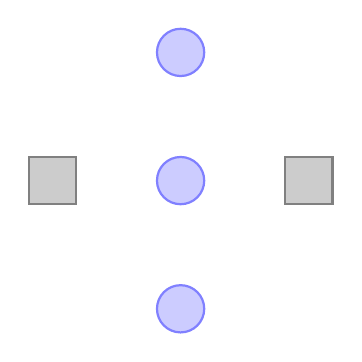
\begin{tikzpicture}[auto, inner sep=0pt, minimum size=6mm,
        place/.style = {circle, draw=blue!50, fill=blue!20, thick},
        transition/.style = {rectangle, draw=black!50, fill=black!20, thick},
        pre/.style = {<-, >=Stealth, semithick},
        post/.style = {->, >=Stealth, semithick}
    ]
        \node[place] (up point) {};
        \node[place] (mid point) [below=of up point] {};
        \node[place] (below point) [below=of mid point]{};
        \node[transition] (left point) [right=of mid point] {};
        \node[transition] (right point) [left=of mid point] {};
    \end{tikzpicture}
\end{document}